\section{Architektur des Microservice}
\label{sec: Architektur des Microservice}
Der Microservice Warenwirtschaft wurde in der Programmiersprache Go\footnote{https:\//golang.org\/doc\/} entwickelt. Go-An-wendungen bestehen aus Packages, in denen die einzelnen Go-Files organisiert sind, Klassen im Sinne der Objektorientierung gibt es nicht. Der Microservice Warenwirtschaft setzt sich aus den neun Packages zusammen, die in der Abbildung \ref{pic:Struktur des Microservice} dargestellt werden. In den nachfolgenden Unterkapiteln \ref{subsec: Presentation Layer} und \ref{subsec: Application Layer} werden die Packages und die darin enthaltenen Go-Files des Presentation  sowie des Application Layers kurz vorgestellt. Go-Files mit der Bezeichnung \texttt{<<Name>>\_test.go} beinhalten Whitebox-Testfälle um die Funktionen der benannten Go-Files zu prüfen. Aus Gründen der Übersichtlichkeit werden diese Files hier nicht explizit aufgeführt. Die weiteren Unterkapitel beschreiben die Schnittstellen, den Persistant Layer sowie die Log-Level, das Admin-Frontend und schließlich die Anpassung des Monolithen,um den Microservice Warenwirtschaft in diesen zu integrieren. 

\begin{figure}[H]
	\centering
	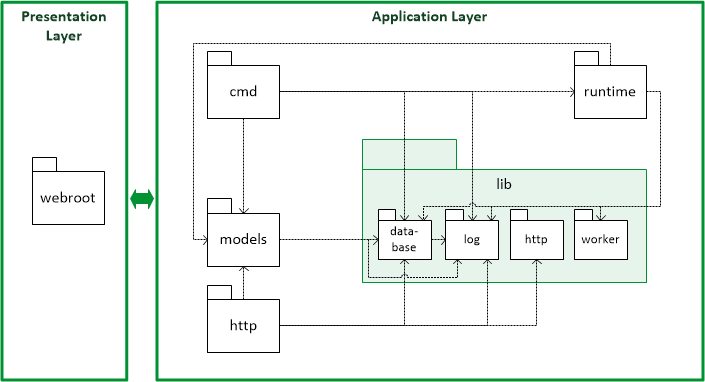
\includegraphics[width=0.95 \textwidth]{./pics/struktur.png}
	\caption{Struktur des Microservice}
	\label{pic:Struktur des Microservice}
\end{figure}

\newpage
\subsection{Schnittstellen zu anderen Microservices}
\label{subsec: Schnittstellen zu anderen Microservices}
Der Microservice Warenwirtschaft weißt drei Schnittstellen\footnote{Da es nicht Teil der übergeordneten Aufgabenstellung war, die Microservices der einzelnen Projektgruppen zu einem lauffähigen Webshop zusammenzufügen, greift der Microservice Warenwirtschaft an diesen Stellen auf Testdaten zurück} zu anderen Microservices auf. Zunächst soll für die Authentifizierung der Benutzer des Admin-Frontends vollständig auf den Microservice Benutzerauthentifizierung zurückgegriffen werden. Anstelle einer Login-Maske weißt das Admin-Frontend deshalb bisher nur einen Icon in Form eines Schlosses auf. Dieser symbolisiert, ob ein Benutzer die passende Berechtigung für das Admin-Front besitzt (Schloss geschlossen) oder nicht (Schloss geöffnet). \par
Weiter benötigt der Microservice Warenwirtschaft Informationen darüber, ob ein Benutzer eine Ware in den Warenkorb gelegt hat und ob eine Bestellung abgeschlossen wurde. So können Waren im Warenkorb für die Bestellung durch andere Benutzer blockiert und die erfolgreich bestellten Waren aus dem Warenbestand gelöscht werden. Diese Funktionalitäten geben eine eine Schnittstelle zu dem Microservice Bestellung vor. \par 
Die dritte Schnittstelle besteht zu dem Microservice Produktkatalog, von welchem die angebotenen Produkte -- die sich dementsprechend im Lager befinden können -- abgefragt werden. Die drei nachfolgenden Listings zeigen die Daten, die von den der Microservices Produktkatalog und Bestellung im JSON-Format erwartet, beziehungsweise an diese ausgegeben werden. 

\begin{lstlisting}[caption=Datenabfrage aus dem Produktkatalog]
{
  "id": <<Int>>,
  "title": "<<Produktname>>"
}
\end{lstlisting}


\begin{lstlisting}[caption=Datenabfrage von der Bestellung (Waren im Warenkorb abgelegt)]
{
  "id": <<Int>>,
  "amount": <<Int>>
}
\end{lstlisting}



\begin{lstlisting}[caption=Datenabfrage von der Bestellung (Waren wurden bestellt)]
{
  "id": <<Int>>,
  "amount": <<Int>>
}
\end{lstlisting}


\newpage
\subsection{Presentation Layer -- Admin-Frontend}
\label{subsec: Presentation Layer}
Der Presentation Layer umfasst alle  Packages, die sich mit der eigentlichen Darstellung der Warenwirtschaft aus der Sicht des Endbenutzers befassen. Im Detail ist dies das Package \textbf{\texttt{webroot}}, welches den statischen Inhalt der Frontends, wie zum Beispiel die HTML-Files und Bilder enthält. \par 
Die Startseite \textit{List} des Admin-Frontends zeigt eine Übersicht aller vorhandenen Produkte mit ihrer Anzahl an Waren (Abbildung \ref{pic:Admin-Frontend -- List}). Letztere wird mit einem Ampelsystem dargestellt, wobei ein vollkommen rot gefärbter Kreis einem Warenbestand von null entspricht und der Kreis mit zunehmender Anzahl an Waren immer mehr grün eingefärbt wird. Zu jeden Produkt kann über den, mit einem  Plus, gekennzeichneten Button Waren hinzugefügt werden. Ein Klick auf das jeweilige Produkt führt zu dessen Produktseite. \par 
Die Produktseiten führen die ID, die Gesamtanzahl an Waren sowie die einzelnen Waren auf (Abbildung \ref{pic:Admin-Frontend -- Produktseite}). Diese können jeweils über den Icon in Form eines Mülleimers manuell gelöscht werden. Auch auf den Produktseiten können über einen, mit einem Plus gekennzeichneten, Button neue Waren hinzugefügt werden. Beim Hinzufügen von neuen Waren sind für diese ein Ablaufdatum, eine Lagerposition sowie ein Kommentar und die Anzahl anzugeben (Abbildung \ref{pic:Admin-Frontend -- Hinzufuegen von Waren}). Um den Microservice auch in anderen Einsatzgebieten, als einem Webshop für Obst- und Gemüse einsetzen zu können, sind hier nur die Felder Lagerposition und Anzahl verpflichtend.  Die Seite \textit{Statistics} gibt letztendlich einen Überblick der gesamten und der durchschnittlichen Waren im Warenbestand.

\begin{figure}[H]
	\centering
	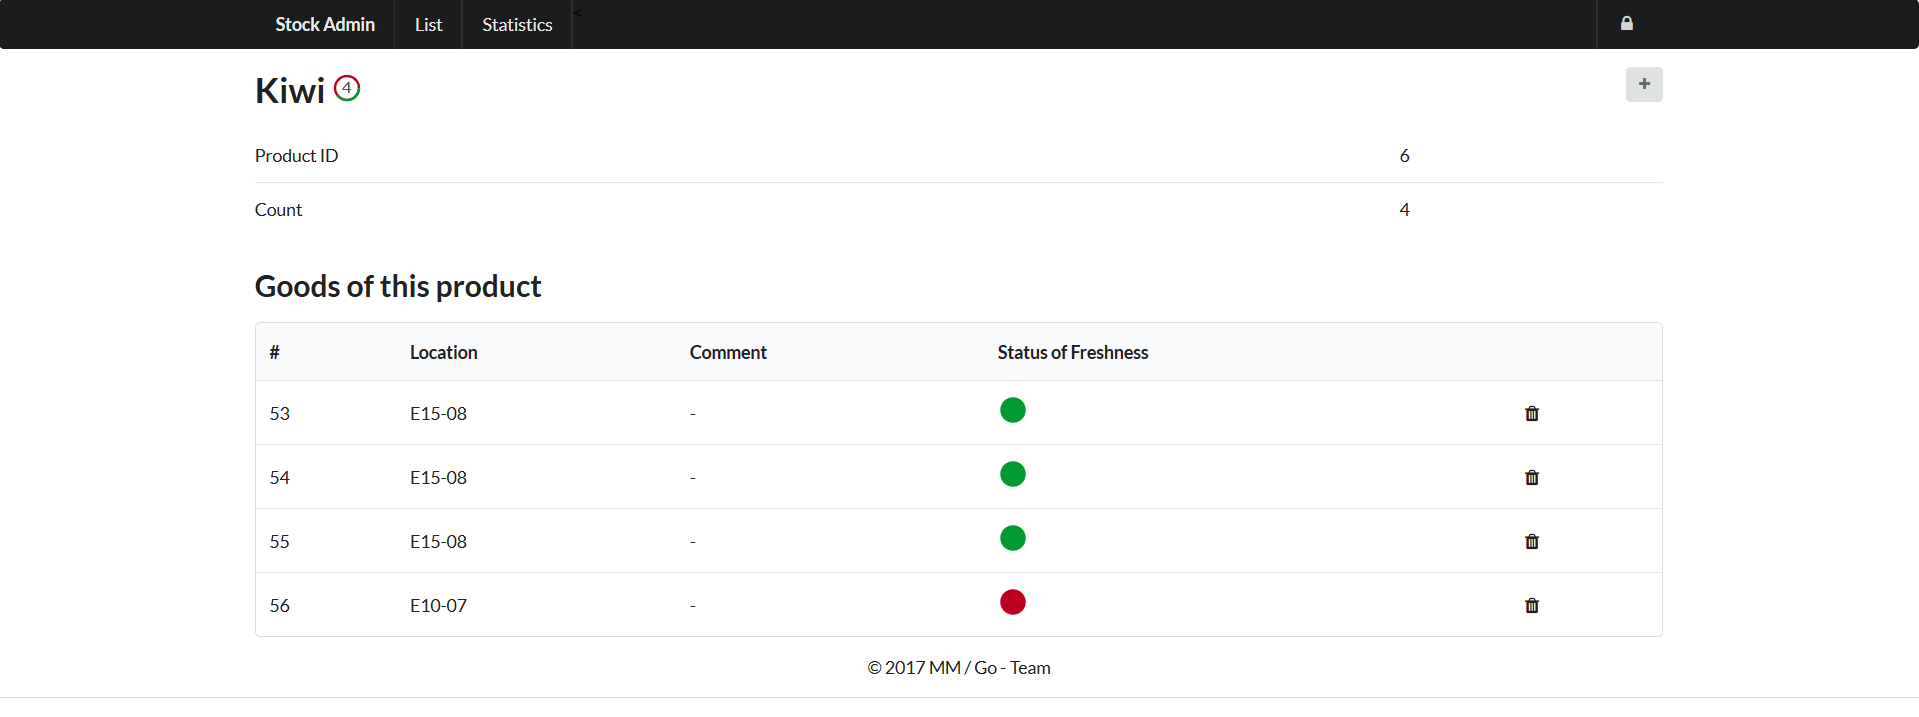
\includegraphics[width=0.65 \textwidth]{./pics/product.png}
	\caption{Admin-Frontend -- Produktseite}
	\label{pic:Admin-Frontend -- Produktseite}
\end{figure}


\begin{figure}[H]
	\centering
	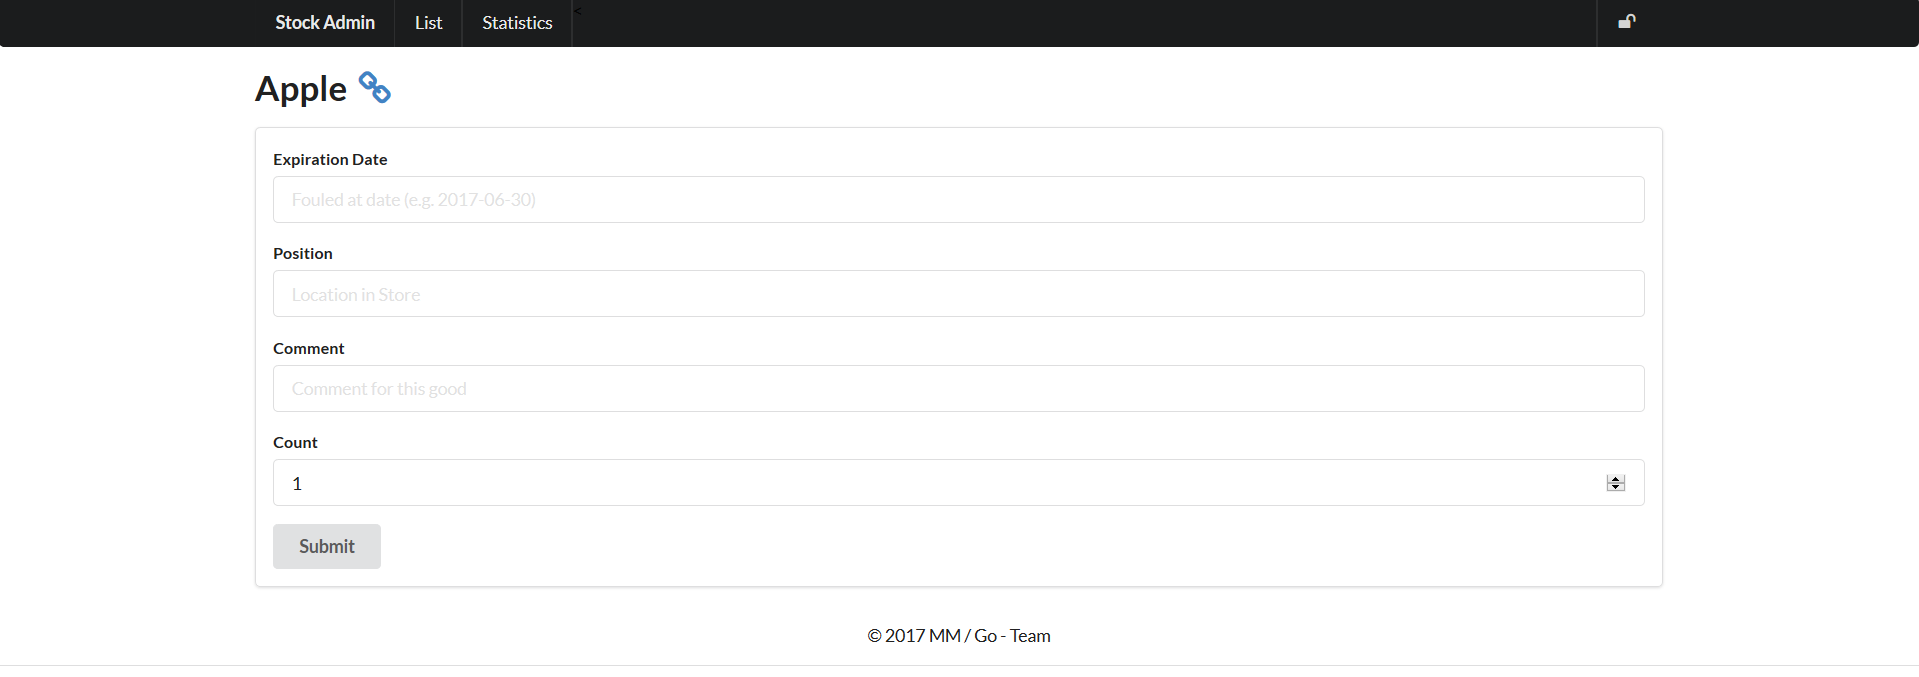
\includegraphics[width=0.65 \textwidth]{./pics/add.png}
	\caption{Admin-Frontend -- Hinzufügen von Waren}
	\label{pic:Admin-Frontend -- Hinzufuegen von Waren}
\end{figure}


\newpage
\subsection{Application Layer}
\label{subsec: Application Layer}
Die Packages des Application Layers umfassen die Logik des Microservice Warenwirtschaft. Sie werden nachfolgend aufgelistet und kurz beschrieben.

\paragraph{cmd:} Go-File main.go, welches die Applixation letztendlich ausführt und alle Angaben zu den Config-Files der Applikation enthält

\paragraph{http:} Go-Files, die die Anwendungslogik (Funktionen) und die API-Routen beinhalten.
	\begin{itemize}
	\item \texttt{bindapi.go}: Funktionen, die für das Binden der URL-Pfade notwendig sind
	\item \texttt{good.go}: Funktionen für das Hinzufügen von Waren zum Warenbestand
	\item \texttt{good\_show.go}: Funktionen für die Auflistung und Zählung der vorhandenen Waren sowie die Feststellung ihrer Verfügbarkeit
	\item \texttt{good\_temp.go}: Hilfsfunktionen, die für die Darstellung des Warenbestandes als Ampel im Kunden-Frontend benötigt werden
	\item \texttt{status.go}: Funktion, die den Status des Microservice abfragt 
	\end{itemize}


\paragraph{models:} Go-Files, die Structs und zugehörige Hilfsfunktionen (hauptsächlich statischen Inhalt des Microservice) beinhalten 
	\begin{itemize}
	\item \texttt{config.go}: Structs mit den Informationen zur Konfiguration des Webservers, der Datenbank und dem Cache-Management sowie Hilfsfunktionen zum Lesen von Config-Files
	\item \texttt{duration.go}: Structs und Hilfsfunktionen zur Definition eines Typs für Zeitangaben
	\item \texttt{good.go}: Structs und Hilfsfunktionen zur Darstellung von Waren, hier werden auch die geforderten Funktionalitäten wie das Blockieren von Waren umgesetzt
	\item \texttt{structstorage}: 
	\end{itemize}


\paragraph{runtime:} Go-Files mit weiteren Hilfsfunktionen
	\begin{itemize}	
	\item \texttt{auth.go}: Hilfsfunktionen zur Prüfung, ob eine Berechtigung für den Zugriff vorliegt
	\item \texttt{cache\_worker.go}: Hilfsfunktionen für das Löschen und Anlegen von Cache-Workers
	\item \texttt{good\_release.go}: Hilfsfunktionen zum Blockieren und Entsperren von Waren
	\item \texttt{productcache.go}: Hilfsfunktionen zum Anlegen eines Caches für Produkte
	\item \texttt{runtime.go}: Übergreifende Hintergrundfunktionalitäten	
	\end{itemize}
	


\newpage
\paragraph{lib:} fasst die vier Packages \texttt{database}, \texttt{http}, \texttt{log} und \texttt{worker} zusammen

	\begin{itemize}
	\item \texttt{database}: Go-File \texttt{database.go} mit Funktionen für das Öffnen und Schließen der Datenbank
	\item \texttt{http}: Go-Files, die die Webserverlogik umgesetzten
		\begin{itemize}
		\item \texttt{io.go}: Funktionen zum Lesen und Schreiben von JSON aus beziehungsweise in HTTP-Pakete
		\item \texttt{permission.go}: Funktionen zur Prüfung der Berechtigung für den Zugriff
		\end{itemize}	
	\item \texttt{log}: Go-File \texttt{log.go}, das den Logger startet und initiiert
	\item \texttt{worker}: Go-File \texttt{worker.go}, dass Funktionen für die Nutzung eines Caches für die Produkte aus dem Produktkatalog (Worker) bereitstellt 
	\end{itemize}


\subsection{Persistant Layer}
Der Persitant Layer umfasst eine SQL-Lite-Datenbank, die im Cache gehalten wird. Die nachfolgende Abbildung \ref{pic:Datenbankmodell des Microservice} zeigt den grundsätzlichen Aufbau der Datenbank. Sie speichert den Warenbestand (stock) in Produkten (product). Jedes Produkt wird mit seiner ID und seinem Namen gehalten, die aus dem Produktkatalog bezogen und in einem Cache zwischengespeichert werden. Zu jedem Produkt gehören wiederum mehrere Waren (good), die eine ID, ein Ablaufdatum und eine Lagerposition besitzen. Dabei kann eine Ware nur zu einem Produkt gehören.

\begin{figure}[H]
	\centering
	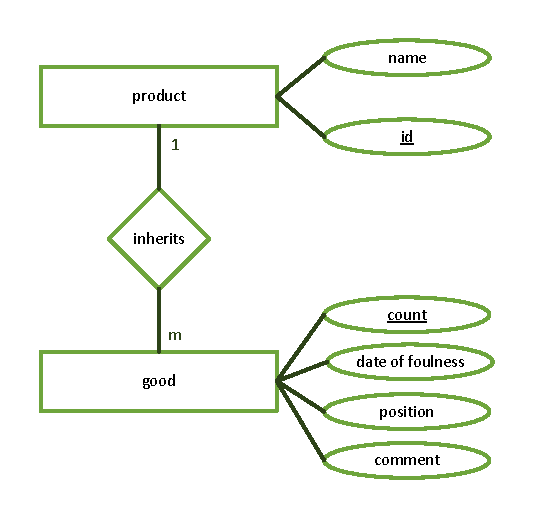
\includegraphics[width=0.65 \textwidth]{./pics/db.pdf}
	\caption{Datenbankmodell des Microservice}
	\label{pic:Datenbankmodell des Microservice}
\end{figure}


\subsection{Integrierte Tests}
\label{subsec: Integrierte Test}
Neben bisherigen Packages, die bereits Whitebox-Tests umfassen, ist in dem Package \textbf{\texttt{test}} ein weiteres Go-File (\texttt{testRest.go}) enthalten. Dieses setzt einen Test des Webservers um, bei dem auf Testdaten eines Produktkataloges zurückgegriffen wird. Mit Hilfe der integrierten Tests kann in der hier beschriebenen Version eine Code-Coverage von 100\% erreicht werden, das heißt jedes Stück Code wird mindestens einmal zur Ausführung gebracht.

\newpage
\subsection{Anpassung des Monolithen}
\label{subsec: Anpassung des Monolithen}
Damit der Microservice Warenwirtschaft durch den bestehenden Monolithen des Webshops Mosh genutzt werden kann, wurden hier dir nachfolgend aufgeführten Änderungen vorgenommen. Zunächst wurde für den Aufruf des Admin-Frontends über die URL des Monolithen \texttt{/stockadmin} das nachfolgende Mapping in der Java-Datei \texttt{HomepageController.java} ergänzt.

\begin{lstlisting}[caption=Datenabfrage von der Bestellung (Waren wurden bestellt), language=Java]
@RequestMapping(value = "/stockadmin", method = RequestMethod.GET)
public String redirect(Model model) {
	return this.STOCKADMINFRONTENDTEMPLATE;
}
\end{lstlisting}

Weiter wurde eine HTML-Datei \texttt{stockadmin.html} zu den statischen Webseiteninhalten des Monolithen hinzugefügt. Diese leitet, wie nachfolgend dargestellt, durch einen Meta-Eintrag direkt auf die Webseite des Microservice Warenwirtschaft weiter. Für den Fall, dass die Umleitung durch den verwendeten Browser nicht unterstützt wird, wurde zudem ein Link auf die Webseite des Microservice integriert.

\begin{lstlisting}[caption=Datenabfrage von der Bestellung (Waren wurden bestellt), language=HTML]
<head th:replace="fragments/skeleton :: head">
	<meta charset="utf-8" />
    <meta http-equiv="refresh" content="5; URL=http://localhost:65000/"/>
    [...]
</head>
\end{lstlisting}
